\documentclass[]{article}
\usepackage{lmodern}
\usepackage{amssymb,amsmath}
\usepackage{ifxetex,ifluatex}
\usepackage{fixltx2e} % provides \textsubscript
\ifnum 0\ifxetex 1\fi\ifluatex 1\fi=0 % if pdftex
  \usepackage[T1]{fontenc}
  \usepackage[utf8]{inputenc}
\else % if luatex or xelatex
  \ifxetex
    \usepackage{mathspec}
    \usepackage{xltxtra,xunicode}
  \else
    \usepackage{fontspec}
  \fi
  \defaultfontfeatures{Mapping=tex-text,Scale=MatchLowercase}
  \newcommand{\euro}{€}
\fi
% use upquote if available, for straight quotes in verbatim environments
\IfFileExists{upquote.sty}{\usepackage{upquote}}{}
% use microtype if available
\IfFileExists{microtype.sty}{%
\usepackage{microtype}
\UseMicrotypeSet[protrusion]{basicmath} % disable protrusion for tt fonts
}{}
\ifxetex
  \usepackage[setpagesize=false, % page size defined by xetex
              unicode=false, % unicode breaks when used with xetex
              xetex]{hyperref}
\else
  \usepackage[unicode=true]{hyperref}
\fi
\hypersetup{breaklinks=true,
            bookmarks=true,
            pdfauthor={},
            pdftitle={},
            colorlinks=true,
            citecolor=blue,
            urlcolor=blue,
            linkcolor=magenta,
            pdfborder={0 0 0}}
\urlstyle{same}  % don't use monospace font for urls
\usepackage{color}
\usepackage{fancyvrb}
\newcommand{\VerbBar}{|}
\newcommand{\VERB}{\Verb[commandchars=\\\{\}]}
\DefineVerbatimEnvironment{Highlighting}{Verbatim}{commandchars=\\\{\}}
% Add ',fontsize=\small' for more characters per line
\newenvironment{Shaded}{}{}
\newcommand{\KeywordTok}[1]{\textcolor[rgb]{0.00,0.44,0.13}{\textbf{{#1}}}}
\newcommand{\DataTypeTok}[1]{\textcolor[rgb]{0.56,0.13,0.00}{{#1}}}
\newcommand{\DecValTok}[1]{\textcolor[rgb]{0.25,0.63,0.44}{{#1}}}
\newcommand{\BaseNTok}[1]{\textcolor[rgb]{0.25,0.63,0.44}{{#1}}}
\newcommand{\FloatTok}[1]{\textcolor[rgb]{0.25,0.63,0.44}{{#1}}}
\newcommand{\ConstantTok}[1]{\textcolor[rgb]{0.53,0.00,0.00}{{#1}}}
\newcommand{\CharTok}[1]{\textcolor[rgb]{0.25,0.44,0.63}{{#1}}}
\newcommand{\SpecialCharTok}[1]{\textcolor[rgb]{0.25,0.44,0.63}{{#1}}}
\newcommand{\StringTok}[1]{\textcolor[rgb]{0.25,0.44,0.63}{{#1}}}
\newcommand{\VerbatimStringTok}[1]{\textcolor[rgb]{0.25,0.44,0.63}{{#1}}}
\newcommand{\SpecialStringTok}[1]{\textcolor[rgb]{0.73,0.40,0.53}{{#1}}}
\newcommand{\ImportTok}[1]{{#1}}
\newcommand{\CommentTok}[1]{\textcolor[rgb]{0.38,0.63,0.69}{\textit{{#1}}}}
\newcommand{\DocumentationTok}[1]{\textcolor[rgb]{0.73,0.13,0.13}{\textit{{#1}}}}
\newcommand{\AnnotationTok}[1]{\textcolor[rgb]{0.38,0.63,0.69}{\textbf{\textit{{#1}}}}}
\newcommand{\CommentVarTok}[1]{\textcolor[rgb]{0.38,0.63,0.69}{\textbf{\textit{{#1}}}}}
\newcommand{\OtherTok}[1]{\textcolor[rgb]{0.00,0.44,0.13}{{#1}}}
\newcommand{\FunctionTok}[1]{\textcolor[rgb]{0.02,0.16,0.49}{{#1}}}
\newcommand{\VariableTok}[1]{\textcolor[rgb]{0.10,0.09,0.49}{{#1}}}
\newcommand{\ControlFlowTok}[1]{\textcolor[rgb]{0.00,0.44,0.13}{\textbf{{#1}}}}
\newcommand{\OperatorTok}[1]{\textcolor[rgb]{0.40,0.40,0.40}{{#1}}}
\newcommand{\BuiltInTok}[1]{{#1}}
\newcommand{\ExtensionTok}[1]{{#1}}
\newcommand{\PreprocessorTok}[1]{\textcolor[rgb]{0.74,0.48,0.00}{{#1}}}
\newcommand{\AttributeTok}[1]{\textcolor[rgb]{0.49,0.56,0.16}{{#1}}}
\newcommand{\RegionMarkerTok}[1]{{#1}}
\newcommand{\InformationTok}[1]{\textcolor[rgb]{0.38,0.63,0.69}{\textbf{\textit{{#1}}}}}
\newcommand{\WarningTok}[1]{\textcolor[rgb]{0.38,0.63,0.69}{\textbf{\textit{{#1}}}}}
\newcommand{\AlertTok}[1]{\textcolor[rgb]{1.00,0.00,0.00}{\textbf{{#1}}}}
\newcommand{\ErrorTok}[1]{\textcolor[rgb]{1.00,0.00,0.00}{\textbf{{#1}}}}
\newcommand{\NormalTok}[1]{{#1}}
\usepackage{graphicx,grffile}
\makeatletter
\def\maxwidth{\ifdim\Gin@nat@width>\linewidth\linewidth\else\Gin@nat@width\fi}
\def\maxheight{\ifdim\Gin@nat@height>\textheight\textheight\else\Gin@nat@height\fi}
\makeatother
% Scale images if necessary, so that they will not overflow the page
% margins by default, and it is still possible to overwrite the defaults
% using explicit options in \includegraphics[width, height, ...]{}
\setkeys{Gin}{width=\maxwidth,height=\maxheight,keepaspectratio}
\setlength{\parindent}{0pt}
\setlength{\parskip}{6pt plus 2pt minus 1pt}
\setlength{\emergencystretch}{3em}  % prevent overfull lines
\providecommand{\tightlist}{%
  \setlength{\itemsep}{0pt}\setlength{\parskip}{0pt}}
\setcounter{secnumdepth}{0}

\date{}

% Redefines (sub)paragraphs to behave more like sections
\ifx\paragraph\undefined\else
\let\oldparagraph\paragraph
\renewcommand{\paragraph}[1]{\oldparagraph{#1}\mbox{}}
\fi
\ifx\subparagraph\undefined\else
\let\oldsubparagraph\subparagraph
\renewcommand{\subparagraph}[1]{\oldsubparagraph{#1}\mbox{}}
\fi

\begin{document}

\section{Goals}\label{goals}

\begin{itemize}
\tightlist
\item
  Learn how Canny edge detector works.
\item
  Understand concepts of Hough line transform.
\item
  Learn about cv2.Canny() and cv2.HoughLines()
\end{itemize}

\section{Theory}\label{theory}

\subsection{Canny Edge Detector}\label{canny-edge-detector}

Developed by John F. Canny, this edge detection algorithm helps reduce
the number of pixels to be processed in an image when extracting
information from it. Following are three criteria to be satisfied in
edge detection-

\begin{enumerate}
\def\labelenumi{\arabic{enumi}.}
\tightlist
\item
  \textbf{Low error rate} - It should detect as many edges as possible
  and ignore all other non-edges.
\item
  \textbf{Localization of edges} - This means that the detected edge
  must not be too far away from the actual edge.
\item
  \textbf{Minimum response} - More than one edges should not be detected
  for one real edge.
\end{enumerate}

Canny edge detection algorithm has five stages, which are explained
below-

\begin{enumerate}
\def\labelenumi{\arabic{enumi}.}
\item
  \textbf{Smoothing} - This includes filtering out any noise present in
  the original image. Noise is undesirable as it can be wrongly detected
  as an edge.
  \href{https://github.com/eyantrainternship/eYSIP_2015_Marker_based_Robot_Localisation/wiki/Image-Filtering}{Gaussian
  filter} is used for this purpose with a convolution mask that is
  generally much smaller than the image itself. The detector's
  sensitivity to noise is inversely proportional to the width of the
  Gaussian mask.
\item
  \textbf{Finding Gradient} - After removing noise, we find intensity
  gradient of the image using a
  \href{https://github.com/eyantrainternship/eYSIP_2015_Marker_based_Robot_Localisation/wiki/Line-Detection:-Part-1}{Sobel}
  operator in x- and y-directions. After this, edge strengths can be
  found by applying the
  \href{https://github.com/eyantrainternship/eYSIP_2015_Marker_based_Robot_Localisation/wiki/Distance-Transformation}{Euclidean
  distance} measure. If Gx and Gy are gradients in x and y-directions
  respectively, then

  edge gradient will be-

  \emph{G = squareRoot( (Gx \^{} 2) + (Gy \^{} 2) )}

  and direction will be -

  \emph{angle = invtan(Gy / Gx)}
\item
  \textbf{Non-maxima suppression} - This step is included to sharpen the
  edges which were blurred in the previous steps. This is done by
  suppressing all gradient values to 0 except the local maxima. This is
  basically an edge-thinning technique.
\item
  \textbf{Double Thresholding} - To determine potential edges,
  \href{https://github.com/eyantrainternship/eYSIP_2015_Marker_based_Robot_Localisation/wiki/Thresholding}{thresholding}
  is performed. In this, edge pixels with a value higher than the
  threshold value are marked as strong, those lesser are suppressed and
  the ones in between as marked as weak. This way, only edges stronger
  than a certain value are preserved.
\item
  \textbf{Hysteresis Tracking} - This step eliminates weak edges or
  streaking. Weak edges are those which are not connected to a strong
  edge. This is performed using BLOB(Binary Large OBject) analysis. In
  this analysis, a pixel and its 8-connected neighbourhood(BLOB) are
  analysed. If at least one strong pixel is identified in a BLOB, then
  it is preserved.
\end{enumerate}

\subsubsection{Example}\label{example}

Consider the following image-

\begin{figure}[htbp]
\centering
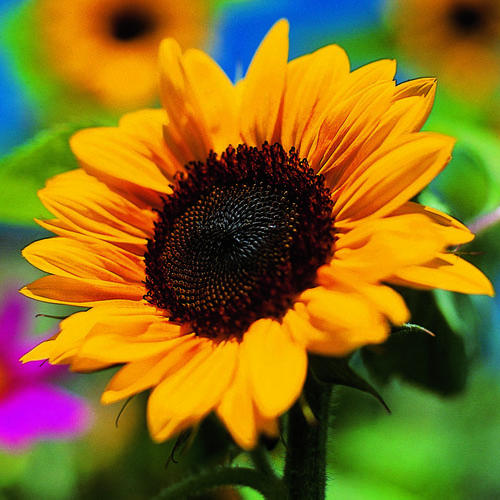
\includegraphics{sunflower.jpg}
\caption{Sunflower}
\end{figure}

On applying Canny edge detection, we get the following result(depicted
using trackbar)-

\begin{figure}[htbp]
\centering
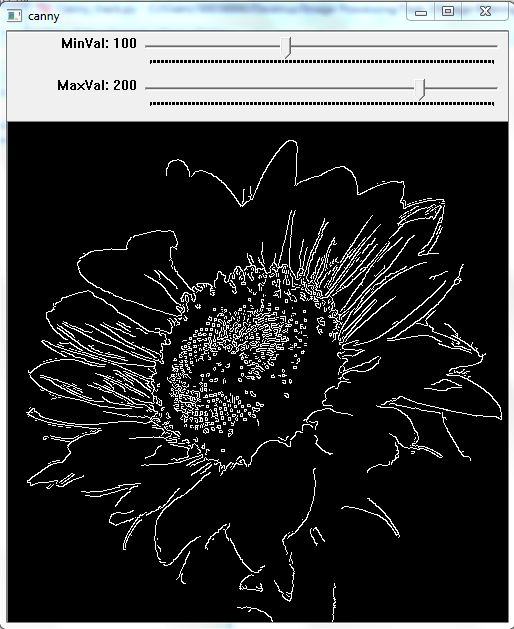
\includegraphics{Canny_trackbar.JPG}
\caption{canny}
\end{figure}

\subsection{Hough lines transform}\label{hough-lines-transform}

The Hough transform is a feature extraction technique.The purpose of the
technique is to find imperfect instances of objects within a certain
class of shapes by a voting procedure. It means that in general, a line
can be detected by finding the number of intersections between curves.

\subsubsection{Working principle}\label{working-principle}

A line in image space can be represented in two ways:\\
\emph{Cartesian coordinate system\\
}Parameter coordinate system\\
Consider the line represented in the polar coordinate system as shown
below:\\
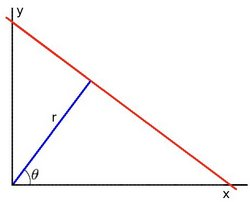
\includegraphics{polar.jpg}\\
Arranging the terms, we can say in general for each point

\includegraphics{xy.png}, we can
define the family of lines passing through the point as :\\ \\

\includegraphics{rcos.png} \\ \\ Hence each
point 
\includegraphics{r0.png}
represents each line that passes through

\includegraphics{xy.png}.

\subsubsection{Function}\label{function}

\texttt{cv2.HoughLines(image,\ rho,\ theta,\ threshold{[},\ lines{[},\ srn{[},\ stn{]}{]}{]})}\\
* \textbf{image} -- 8-bit, single-channel binary source image. The image
may be modified by the function.\\
* \textbf{lines} -- Output vector of lines. Each line is represented by
a two-element vector

\includegraphics{r0.png} .

\includegraphics{rho.png} is the
distance from the coordinate origin (0,0) (top-left corner of the
image). 
\includegraphics{thetha.png}
is the line rotation angle in radians. \\
* \textbf{rho} -- Distance resolution of the accumulator in pixels.\\
 * \textbf{theta} -- Angle resolution of the accumulator in radians.\\
 * \textbf{threshold} --Accumulator threshold parameter. Only those lines are returned that get
enough votes (\textgreater{}threshold). \\
* \textbf{srn} -- For the multi-scale Hough transform, it is a divisor for the distance resolution
rho . The coarse accumulator distance resolution is rho and the accurate
accumulator resolution is rho/srn . If both srn=0 and stn=0 , the
classical Hough transform is used. Otherwise, both these parameters
should be positive. \\
* \textbf{stn} -- For the multi-scale Hough transform, it is a divisor for the distance resolution theta.

\section{Code}\label{code}

\subsection{Canny Edge Detection}\label{canny-edge-detection}

The main function used is-

\begin{verbatim}
cv2.Canny(src, threshold1, threshold2[, edges[, apertureSize[, L2gradient]]])
\end{verbatim}

\textbf{Parameters}-

\begin{itemize}
\tightlist
\item
  \textbf{src}- Single-channel 8-bit input image
\item
  \textbf{threshold1}- First threshold for the hysteresis procedure
\item
  \textbf{threshold2}- Second threshold for the hysteresis procedure
\item
  \textbf{edges}- Output edge map; it has the same size and type as src
\item
  \textbf{apertureSize}- aperture size for the Sobel() operator
\item
  \textbf{L2gradient}- Flag indicating whether L2 or L1 norm should be
  used to calculate the image gradient magnitude
\end{itemize}

We shall now have a look at a simple canny edge detection code.

\begin{Shaded}
\begin{Highlighting}[]
\CommentTok{#Import opencv}
\ImportTok{import} \NormalTok{cv2}

\CommentTok{#Read the image}
\NormalTok{img }\OperatorTok{=} \NormalTok{cv2.imread(}\StringTok{'example.jpg'}\NormalTok{)}

\CommentTok{#Canny edge detect}
\NormalTok{edges }\OperatorTok{=} \NormalTok{cv2.Canny(img, }\DecValTok{100}\NormalTok{, }\DecValTok{200}\NormalTok{)}

\CommentTok{#Display image}
\NormalTok{cv2.imshow(}\StringTok{'Canny'}\NormalTok{, edges)}

\CommentTok{#Exit}
\NormalTok{cv2.waitKey(}\DecValTok{0}\NormalTok{)}
\NormalTok{cv2.destroyAllWindows()}
\end{Highlighting}
\end{Shaded}

\newpage
\subsection{Hough Line Transform}\label{hough-line-transform}

\begin{verbatim}
 #Import modules 
 import cv2   
 import numpy as np
 import matplotlib.pyplot as plt

 #Read the image   
 img = cv2.imread('road3.jpg')

 gray = cv2.cvtColor(img,cv2.COLOR_BGR2GRAY)
 edges = cv2.Canny(gray,220,150,apertureSize = 3)


 lines = cv2.HoughLines(edges,1,np.pi/180,90,10)

 for rho,theta in lines[0]:
      a = np.cos(theta)
      b = np.sin(theta)
      x0 = a*rho
      y0 = b*rho
      x1 = int(x0 + 1000*(-b))
      y1 = int(y0 + 1000*(a))
      x2 = int(x0 - 1000*(-b))
      y2 = int(y0 - 1000*(a))

      cv2.line(img,(x1,y1),(x2,y2),(0,0,255),2)

cv2.imshow('canny',edges)
cv2.imshow('Hough',img)
cv2.waitKey(0)
cv2.destroyAllWindows()
\end{verbatim}

\begin{figure}[htbp]
\centering
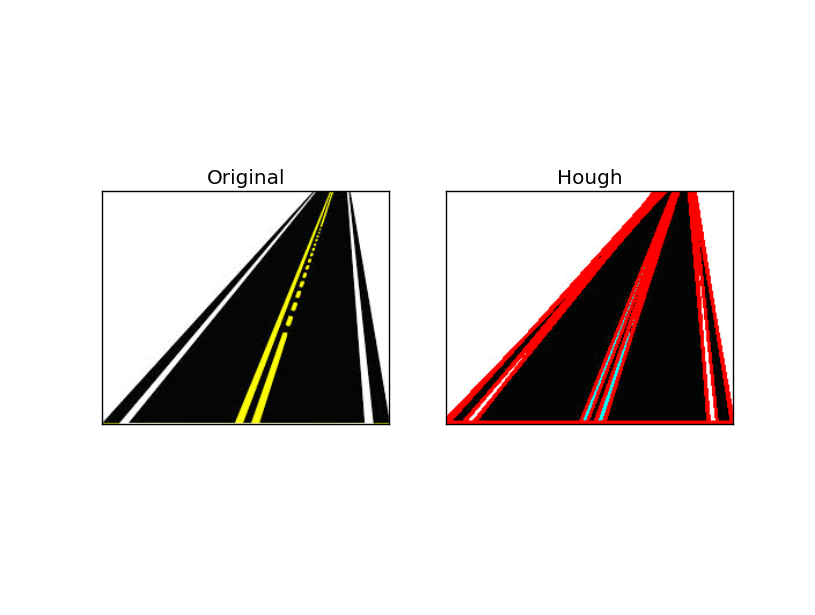
\includegraphics{hough.png}
\caption{Output Image}
\end{figure}

\newpage
\section{Resources}\label{resources}

\begin{itemize}
\tightlist
\item
  \href{http://www.cse.iitd.ernet.in/\textasciitilde{}pkalra/csl783/canny.pdf}{cse.iitd - pdf}
\item
  \href{http://dasl.mem.drexel.edu/alumni/bGreen/www.pages.drexel.edu/\_weg22/can\_tut.html}{Canny edge detection}
\item
  \href{http://opencv-python-tutroals.readthedocs.org/en/latest/py\_tutorials/py\_imgproc/
  py\_canny/py\_canny.html}{Canny - opencv-python tutorials}
\item
  \href{http://en.wikipedia.org/wiki/Canny\_edge\_detector}{Canny edge detector - Wiki}
\item
  \href{http://docs.opencv.org/modules/imgproc/doc/feature\_detection.html}{Opencv docs}
\end{itemize}

\end{document}
